
\documentclass[conference,final,12pt,]{IEEEtran}


\ifCLASSINFOpdf

\else
\texttt{new times roman}
\fi



\usepackage{graphicx}
% We will generate all images so they have a width \maxwidth. This means
% that they will get their normal width if they fit onto the page, but
% are scaled down if they would overflow the margins.
\makeatletter
\def\maxwidth{\ifdim\Gin@nat@width>\linewidth\linewidth
\else\Gin@nat@width\fi}
\makeatother
\let\Oldincludegraphics\includegraphics
\renewcommand{\includegraphics}[1]{\Oldincludegraphics[width=\maxwidth]{#1}}

\usepackage[unicode=true]{hyperref}
\usepackage[spanish]{babel}
\usepackage[utf8]{inputenc} 
\usepackage[T1]{fontenc}
%\usepackage{newtxmath,newtxtext}
\usepackage{bookman}
\usepackage{lmodern}
\usepackage{natbib}
\bibliographystyle{jss}
\renewcommand{\spanishtablename}{Tabla}

\hypersetup{
            pdftitle={Bare Demo of IEEEtran.cls for IEEE Conferences},
            pdfkeywords={Diversidad, Zonación, Similitud, Manglar, Bosque aluvial},
            pdfborder={0 0 0},
            breaklinks=true, 
            colorlinks,
            citecolor=red,
            urlcolor=blue}
\urlstyle{same}  % don't use monospace font for urls

% Pandoc toggle for numbering sections (defaults to be off)
\setcounter{secnumdepth}{0}

% Pandoc syntax highlighting


% Pandoc header

\providecommand{\tightlist}{%
  \setlength{\itemsep}{0pt}\setlength{\parskip}{0pt}}

%% END MY ADDITIONS %%


\hyphenation{op-tical net-works semi-conduc-tor}

\begin{document}


%
% paper title
% Titles are generally capitalized except for words such as a, an, and, as,
% at, but, by, for, in, nor, of, on, or, the, to and up, which are usually
% not capitalized unless they are the first or last word of the title.
% Linebreaks \\ can be used within to get better formatting as desired.
% Do not put math or special symbols in the title.
\title{Comparación de la diversidad de tres parcelas y los cambios que presentan en sus estructuras en un bosque de manglar y un bosque aluvial de la costa del Urabá Antioqueño}

% author names and affiliations
% use a multiple column layout for up to three different
% affiliations

\author{

%% ---- classic IEEETrans wide authors' list ----------------
 % -- end affiliation.wide
%% ----------------------------------------------------------



%% ---- classic IEEETrans one column per institution --------
 %% -- beg if/affiliation.institution-columnar
\IEEEauthorblockN{
  %% -- beg for/affiliation.institution.author
Cristian Gañan T %% -- end for/affiliation.institution.author
}
\IEEEauthorblockA{Dep. Ciencias Forestales\\
U Nacional de Colombia\\
Medelín, Antioquia
\\ccganant@unal.edu.co
}
\and
\IEEEauthorblockN{
  %% -- beg for/affiliation.institution.author
Camilo Cruz S %% -- end for/affiliation.institution.author
}
\IEEEauthorblockA{Dep. Ciencias Forestales\\
U Nacional de Colombia\\
Medellín, Antioquia
\\cacruzs@unal.edu.co
}
\and
\IEEEauthorblockN{
  %% -- beg for/affiliation.institution.author
Juan Caicedo G %% -- end for/affiliation.institution.author
}
\IEEEauthorblockA{Dep. Ciencias Forestales\\
U Nacional de Colombia\\
Medellín, Antioquia
  %% -- beg for/affiliation.institution.author
\\jpcaicedog@unal.edu.co
 %% -- end for/affiliation.institution.author
}
 %% -- end for/affiliation.institution
 %% -- end if/affiliation.institution-columnar
%% ----------------------------------------------------------





%% ---- one column per author, classic/default IEEETrans ----
 %% -- end if/affiliation.institution-columnar
%% ----------------------------------------------------------

}

% conference papers do not typically use \thanks and this command
% is locked out in conference mode. If really needed, such as for
% the acknowledgment of grants, issue a \IEEEoverridecommandlockouts
% after \documentclass

% for over three affiliations, or if they all won't fit within the width
% of the page, use this alternative format:
%
%\author{\IEEEauthorblockN{Michael Shell\IEEEauthorrefmark{1},
%Homer Simpson\IEEEauthorrefmark{2},
%James Kirk\IEEEauthorrefmark{3},
%Montgomery Scott\IEEEauthorrefmark{3} and
%Eldon Tyrell\IEEEauthorrefmark{4}}
%\IEEEauthorblockA{\IEEEauthorrefmark{1}School of Electrical and Computer Engineering\\
%Georgia Institute of Technology,
%Atlanta, Georgia 30332--0250\\ Email: see http://www.michaelshell.org/contact.html}
%\IEEEauthorblockA{\IEEEauthorrefmark{2}Twentieth Century Fox, Springfield, USA\\
%Email: homer@thesimpsons.com}
%\IEEEauthorblockA{\IEEEauthorrefmark{3}Starfleet Academy, San Francisco, California 96678-2391\\
%Telephone: (800) 555--1212, Fax: (888) 555--1212}
%\IEEEauthorblockA{\IEEEauthorrefmark{4}Tyrell Inc., 123 Replicant Street, Los Angeles, California 90210--4321}}




% use for special paper notices
%\IEEEspecialpapernotice{(Invited Paper)}




% make the title area
\maketitle

% As a general rule, do not put math, special symbols or citations
% in the abstract
\begin{abstract}
La diversidad siendo uno de los parámetros más importantes que se usan
para entender la dinámica de los ecosistemas y como está afecta a la
estructura de los bosques y la dinámica de sus comunidades, a partir de
esto se analizó la diversidad y el cambio en la estructuras de 3
parcelas circulares (62, 69 y 70) de \textbf{\(500 \ m^2\)} ubicadas en el Urabá
Antioqueño, con el fin de identificar si hacen parte de la misma
comunidad o no; se utilizaron los índices de diversidad alfa y beta, y
diferentes modelos como de riqueza esperada, de Valor de importancia y
diámetricos . Según los resultados de los índices alfa se pudo llegar a
la conclusión de que la parcela 69 tiene la mayor diversidad según las
pruebas de Shannon, Simpson y Alfha; de igual forma se encontró que la
parcela 69 es diferente a las parcelas 62 y 70 por medio de los índices
beta (Morisita y Sorensen), por lo tanto se podría pensar que existe una
zonación a través de las 3 parcelas, ubicando a la 62 y 70 más cercanas
a la costa. Además se determinó que la especie con más peso en el índice
de valor de importancia para las tres parcelas fue \emph{Rhizophora
Mangle}, con una riqueza esperada según Jacknife de 14 especies.
\end{abstract}

% keywords
\begin{IEEEkeywords}
Diversidad; Zonación; Similitud; Manglar; Bosque aluvial
\end{IEEEkeywords}

% use for special paper notices



% make the title area
\maketitle

% no keywords

% For peer review papers, you can put extra information on the cover
% page as needed:
% \ifCLASSOPTIONpeerreview
% \begin{center} \bfseries EDICS Category: 3-BBND \end{center}
% \fi
%
% For peerreview papers, this IEEEtran command inserts a page break and
% creates the second title. It will be ignored for other modes.
\IEEEpeerreviewmaketitle


\hypertarget{introducciuxf3n}{%
\section{Introducción}\label{introducciuxf3n}}

Los estudios de diversidad han sido catalogados desde el punto de vista
científico como una ayuda enorme para entender la dinámica de los
distintos ecosistemas, también como sinónimo de ``variedad de vida''
\citep{A}. Existen dos áreas principales en las cuales los estudios y
medidas de diversidad han tenido una gran aplicación, se pueden ver
entonces desde el punto de vista de la conservación la cual está basada
en que las comunidades ricas en especies son mejores que las pobres en
estas, y desde el punto de vista de la supervisión ambiental donde se
tienen en cuenta los efectos adversos en la reducción de la diversidad o
en un cambio de forma de la distribución de abundancia de las
especies\citep{B}. En los agrosistemas mantener o restaurar altos niveles
de diversidad, aumenta su resistencia al cambio climático, apoya la
provisión equilibrada de servicios ecosistémicos y contribuye a la
conectividad del hábitat \citep{C}.

La diversidad como una medida tangible es obtenida por medio de diversos
índices que además de dar un valor de la diversidad en cualquier
comunidad también expresa comportamientos en las comunidades tales como
la riqueza, dominancia, la equidad, la abundancia relativa, similitud y
disimilitud, entre otros; los cuales son importantes de conocer, ya
pueden decir que tan resistente puede ser la comunidad a periodos de
tensión como hídricos, de temperatura, enfermedades o cualquier otra
causada de forma natural o antrópica\citep{D}. Por otra parte, \citep{E}
formalizó matemáticamente el concepto de diversidad de especies y
planteó tres componentes cuantificables: alfa (\(\alpha\)), beta
(\(\beta\)) y gamma (\(\gamma\)), los cuales son importantes a la hora
de querer conocer y diferenciar la diversidad y estructura de distintas
comunidades, los índices alfa han sido importantes en conocer la
diversidad dentro de una comunidad (En este caso parcela), los beta para
conocer y comparar la diversidad entre varias comunidades y corroborar
el reemplazamiento de especies entre una comunidad y otra (parcelas para
este estudio), generalmente, la diversidad alfa se evalúa con la riqueza
de especies presentes en una comunidad y la diversidad beta con índices
que miden la disimilitud en la composición de especies entre las
comunidades \citep{G}.

La importancia de la determinación de los diferentes índices, está en
diferenciar entre tipos de bosques y conocer los diferentes cambios
ambientales para explicar el reemplazamiento de especies y el cambio en
la estructura de los mismos, se entiende que la estructura de los
bosques está relacionada con la diversidad, pero también con condiciones
ambientales como el clima y el suelo\citep{H}, y que dicha estructura
tiende a responder a las exigencias de las especies \citep{J} que hacen
que esta cambie continuamente \citep{I}, entonces conocer las diferentes
diversidades de los tipos de bosques y compararlas da una idea acerca de
qué tan diversos son y cual de ellos representa una mayor complejidad
estructural teniendo en cuenta su diversidad y factores bióticos y
abióticos que la controlan. La estructura observada en cada situación
particular es la mejor respuesta del ecosistema a sus propias
características \citep{F}.

En este artículo se tiene como objetivo comparar la diversidad entre
parcelas que vienen de dos tipos de bosques en el Urabá Antioqueño
(manglares y bosques inundables), como esta afecta en la estructura de
la comunidad, con la ayuda de distribuciones de diámetro y altura, para
conocer la estructura que maneja y su distribución de especies, para
poder decidir si las diferentes parcelas en estudio pertenecen a una
misma comunidad o si se encuentran en comunidades diferentes, todo con
la ayuda de los diferentes índices de diversidad y componentes de la
estructura. Además de análisis como el índice de valor de
importancia(IVI) que ayudan a cuantificar la importancia de las
diferentes especies en las parcelas, y otros que nos permitirán realizar
esta comparación y entender la zonación, es decir el cambio que
presentan las especies más importantes a lo largo de un gradiente de las
condiciones ambientales, teniendo en cuenta las preferencias ecológicas
de dichas especies.

\hypertarget{muxe9todos}{%
\section{Métodos}\label{muxe9todos}}

Las parcelas que se comparan en el presente estudio fueron tomadas de
una base de datos realizada por Urrego, Molina y Suárez tomadas dos
tipos de bosques (Manglares y bosques Aluviales) en el Urabá Antioqueño
con el fin de determinar la variabilidad de la vegetación a lo largo de
las costas, por medio de la evaluación de la estructura, composición
florística y atributos ambientales de los manglares. Según los
autores\citep{AB} el trabajo de campo se realizó de septiembre de 2009 a
enero. 2010, y se trazaron 87 parcelas circulares de 500 m2 para
muestreo. En cada parcela, se midió el diámetro a la altura del pecho
(DAP) y altura total de todos los árboles con DAP superior a 5 cm, e
identificando cada árbol para los individuos con DAP entre 2.5 y 5 cm,
para las parcelas muestreadas por tipo de manglar se basaron en una
exploración de muestreo previo (se establecieron cinco parcelas y se
midieron en cada tipo de bosque). Además se tomaron datos de salinidad e
inundación de cada parcela. En este estudio solo se tendrán en cuenta
las parcelas 62, 69 y 70, para la cuales se hallaron índices para
diversidad Alfa y Beta con el fin de comparar la diversidad entre las
parcelas ya mencionadas. Para el cálculo de la diversidad alfa se
utilizaron los índices de diversidad de Shannon, La diversidad de
Simpson (1-D), la diversidad alfa de fisher y el índice de riqueza de
Margalef y para el cálculo de diversidad Beta se usaron los índices de
Sorensen y Morishita. Cálculos que fueron realizados a través del
software R versión 3.6.1

Las parcelas que se comparan en el presente estudio fueron tomadas de
una base de datos realizada por Urrego, Molina y Suárez tomadas dos
tipos de bosques (Manglares y bosques Aluviales) en el Urabá Antioqueño
con el fin de determinar la variabilidad de la vegetación a lo largo de
las costas, por medio de la evaluación de la estructura, composición
florística y atributos ambientales de los manglares. Según los
autores\citep{AB} el trabajo de campo se realizó de septiembre de 2009 a
enero. 2010, y se trazaron 87 parcelas circulares de 500 m2 para
muestreo. En cada parcela, se midió el diámetro a la altura del pecho
(DAP) y altura total de todos los árboles con DAP superior a 5 cm, e
identificando cada árbol para los individuos con DAP entre 2.5 y 5 cm,
para las parcelas muestreadas por tipo de manglar se basaron en una
exploración de muestreo previo (se establecieron cinco parcelas y se
midieron en cada tipo de bosque). Además se tomaron datos de salinidad e
inundación de cada parcela. En este estudio solo se tendrán en cuenta
las parcelas 62, 69 y 70, para la cuales se hallaron índices para
diversidad Alfa y Beta con el fin de comparar la diversidad entre las
parcelas ya mencionadas. Para el cálculo de la diversidad alfa se
utilizaron los índices de diversidad de Shannon, La diversidad de
Simpson (1-D), la diversidad alfa de fisher y el índice de riqueza de
Margalef y para el cálculo de diversidad Beta se usaron los índices de
Sorensen y Morishita. Cálculos que fueron realizados a través del
software R versión 3.6.1

\textbf{Índices de diversidad alfa.} Las medidas de diversidad más
ampliamente usadas son los índices de la teoría de la información. Estos
índices se basan en la lógica de que la diversidad o la información, en
un sistema natural pueden ser medidos de un modo similar a la
información contenida en un código o mensaje. Algunos de estos índices
derivados de la teoría de la información son los índices de Shannon y
Simpson \citep{B}. \textbf{Margalef.} El índice de riqueza de especies de
Margalef transforma el número de especies por muestra a una proporción a
las cuales las especies son añadidas por expansión de la
muestra\citep{N}, es decir, a mayor número de muestras se espera mayor
riqueza de especies. Para el cálculo se usa \(S-1/Ln(N)=Dmr\), Donde
\(Dmr=0\) indica que solo existe una especie en la muestra.\citep{N}.
\textbf{Shannon y Simpson.} El índice de Shannon refleja la
heterogeneidad de una comunidad sobre la base de dos factores: el número
de especies presentes y su abundancia relativa. La diversidad máxima
(Hmax= lnS) se alcanza cuando todas las especies están igualmente
presentes. Un índice de homogeneidad asociado a esta medida de
diversidad puede calcularse como el cociente H/Hmax=H/lnS, que será 1 si
todas las especies que componen la comunidad tienen igual probabilidad
\citep{L}. La definición más simple del índice de Simpson es la
probabilidad de que dos individuos extraídos al azar de una comunidad
pertenezcan a la misma especie\citep{K}, es una medida de dominio, pero
también puede ser convertido en medida de diversidad restándole a su
resultado 1, este se puede establecer como la probabilidad de que dos
especies tomadas al azar de una comunidad sean diferentes, entonces el
criterio de diversidad está determinado por el número de pares de
individuos que difieren en especie\citep{M}, el índice está fuertemente
recargado hacia las especies más raras de la muestra\citep{B}.
\textbf{Alfa de fisher.} Es un modelo de abundancia a partir de una
serie logarítmica que solo toma en cuenta el número de especies (S) y el
número total de individuos(N)\citep{P}. Este índice funciona mejor con
datos donde todas las especies tienen una baja abundancia\citep{Q}. el
alfa de Fisher es una herramienta muy eficaz para estimar la magnitud de
las diferencias esperadas en términos de la riqueza entre regiones con
tamaños de muestra más grandes, con base en un número limitado de
individuos.\citep{R}. Para este caso se tomó un número de 100 individuos.

\textbf{Índices beta.} El concepto de diversidad \(\beta\) tiene gran relevancia
en ecología y biogeografía para comprender, cuantificar y valorar la
diversidad biológica, y puede considerarse como un concepto clave para
entender el funcionamiento de los ecosistemas, para la conservación de
la biodiversidad y para el manejo de los ecosistemas \citep{O}, Whitaker
la define como ``la magnitud de cambio en la composición de las especies
a lo largo de un gradiente ambiental o entre diferentes comunidades en
un paisaje'' (Whittaker, 1977). La forma más sencilla de medir la
diversidad Beta es mediante el uso de coeficientes de similaridad
\citep{B}, entre estos se pueden encontrar los índices de Sorensen y
Morisita-Horn que son medidas cuantitativas que tienen en cuenta la
abundancia relativa. En virtud de que la similitud es una construcción
cualitativa humana, no tiene una definición matemática precisa. No
obstante, el medir `la similitud' depende de índices cuantitativos
diseñados para el propósito, y en la práctica, podemos esperar que los
índices de la similitud cumplan con criterios razonables para su
comportamiento matemático \citep{S}

\textbf{Riqueza esperada.} Cuando se hacen inventarios forestales con el
fin de determinar la biodiversidad de algún tipo de sistema, siempre se
tiene el problema de no muestrear la cantidad total de especies que se
pueden encontrar en dicho espacio, y al mismo tiempo para poder comparar
entre comunidades se necesitan las mismas muestras en ambos sitios, por
lo tanto la rarefacción se impuso como un método ampliamente utilizado
\citep{Z}, y por otra parte los métodos no paramétricos como el Jacknife
\citep{AA} para dar solución a este problema y determinar la riqueza
esperada de algún lugar en estudio.\\
\textbf{Jacknife.} Modelo usado para la estimación de la
riqueza\citep{X}, se basa en el número de especies raras y existen dos
modelos Jack 1 y Jack 2, para este estudio se usa solo Jack 1 que tiene
en cuenta el número de especies presentes en una sola unidad de
muestreo\citep{Y} \textbf{Rarefacción.} Es un método que se usa para
obtener las especies esperadas. Es importante ya que se estima en base a
un numero estandar de muestras, es decir teniendo en cuenta que todas
las comunidades estudiadas tuvieran el mismo número de
individuos.\citep{B}

\textbf{Número efectivo de especies.} Los números efectivos de especies
(medidas de diversidad verdadera) permiten obtener una interpretación
intuitiva y fácilmente comparable de la diversidad de especies.\citep{V}.
Una de las principales ventajas del cálculo del número de especies
efectivas es la facilidad con la cual podemos evaluar directamente la
magnitud de los cambios en la diversidad entre comunidades.\citep{W}, lo
cual no es posible con los índices tradicionalmente utilizados. Desde el
enfoque de la ecología, la diversidad de especies es una propiedad
relacionada con la estructura de las comunidades, que puede definirse
como el recíproco de un promedio de las abundancias relativas de las
especies. El valor de este recíproco es el número máximo posible de
especies que podrían coexistir en una comunidad, si todas ellas tuvieran
la misma abundancia, es decir, el número efectivo de especies en la
comunidad \citep{W}. Se halla con la fórmula propuesta por Jost, que
cambia según el valor del parámetro q determina qué tanto influyen las
especies comunes o las especies raras en la medida de la diversidad, y
puede tomar cualquier valor que el usuario estime apropiado. Si q = 0 el
valor de la ecuación equivale a la riqueza de especies, si q = 1 es
equivalente al exponencial del índice de Shannon, y si q=2 es
equivalente al índice de dominancia de Simpson.

\textbf{Medidas para entender el comportamiento de la estructura.}
\textbf{\emph{Índice de valor de importancia(IVI)}}. Desarrollado por
Curtis \& McIntosh\citep{T}, es un índice que permite comparar el peso o
valor ecológico relativo de las especies dentro de la comunidad y
consiste en la sumatoria de los valores relativos de densidad,
frecuencia y dominancia.\citep{U}. Se asumió una sola comunidad entre las
tres parcelas para este índice.

\textbf{\emph{Modelos de distribución diamétrica.}} Las distribuciones
diamétricas son las relaciones del diámetro con sus frecuencia absoluta
respectiva, son muy importantes para la caracterización de por ejemplo
los diferentes interacciones entre especies de luz y de sombra, así como
irregularidades debidas a la historia del bosque, a la geomorfología, a
la topografía y al comportamiento de algunas especies (AE), en este
sentido, se eligieron algunas de los modelos más conocidos para ajustar
los datos, Weibull, Gamma, Log-normal y Beta.

\hypertarget{resultados-y-discusiuxf3n}{%
\section{Resultados y discusión}\label{resultados-y-discusiuxf3n}}

Se quiere y se necesita medir la diversidad porque, como en cualquier
ciencia, las medidas permiten describir los componentes del sistema bajo
estudio, hacer comparaciones entre sistemas y porque representan la
materia prima para generar teorías \citep{U}

\begin{table}

\caption{\label{tab:unnamed-chunk-2}indices alfa}
\centering
\begin{tabular}[t]{l|r|r|r|r}
\hline
Parcela & Margalef & Shannon & Simpson & Fisher\\
\hline
62 & 0.2227848 & 0.0616067 & 0.0222194 & 2.042935\\
\hline
69 & 1.1476553 & 1.1471140 & 0.6213018 & 6.370040\\
\hline
70 & 0.5824134 & 0.3795349 & 0.1789802 & 3.945655\\
\hline
\end{tabular}
\end{table}

En la \textbf{Tabla I} se pueden observar los resultados de los
diferentes índices para la diversidad alfa, los cuales dan una
cuantificación de la diversidad por separado de cada parcela en el
estudio. En el índice de riqueza de Margalef se puede observar que estas
tres parcelas tienen una baja riqueza de especies, ya que cuentan con un
valor por debajo de 2 \citep{B},sin embargo se pueden comparar entre
ellas siendo la parcela 69 con mayor diversidad; esta tendencia a una a
baja riqueza de especies en estas diferentes parcelas, era de esperarse
ya que son comunidades que tienen unas restricciones ambientales
importantes, ya sea por la salinidad en los manglares\citep{AD} o por los
periodos de inundación a los que se ven sometidos los bosques aluviales,
de igual forma a la tendencia que tienen estos tipos de bosques
(manglares) a formar rodales puros de especies; en este caso se puede
evidenciar con los datos que la parcela 62, la cual tiene una riqueza de
especies muy baja y una diversidad dada por el índice de simpson
igualmente baja (Alta dominancia) es debido a la alta presencia y
dominancia de la especie \emph{Rhizophora Mangle}, según \citep{Z}, en
los manglares la especie mejor conocida es el mangle rojo
(\emph{Rhizophora Mangle}) por lo tanto se puede pensar que la parcela
62 hace referencia a un bosque que posiblemente es el que está expuesto
a una salinidad más alta de las tres parcelas, estando más cerca a la
costa y se podría catalogar como manglar.

Teniendo en cuenta lo anterior con la realización de los demás índices
de diversidad (Shannon, Simpson y alfa de fisher)(\textbf{Tabla I}) se
puede verificar que la diversidad aumenta (sin ser alta) según el alfa
fisher desde la parcela 62 que es la de más baja diversidad, hacia la
parcela 70 y terminando con la parcela 69, esto debido al mayor número
de especies y una dominancia no tan marcada en esta última parcela,
comprobando así que entre el índice de alfa y el índice de dominancia de
Simpson hay una relación inversa, es decir, a mayor índice de diversidad
alfa menor índice de dominancia de simpson, como se puede ver en la
\textbf{Tabla I}, la parcela 69 cuenta con el índice más alto de alfa de
fisher(6,37) y el índice más bajo de dominancia de Simpson(1-0,62=0,38)
entre las tres parcelas. Esto concuerda con lo expuesto en el libro de
ecología de Guariguata donde se dice que las comunidades más
heterogéneas en ecosistemas en contacto directo con el agua, se
encuentran más alejados del mar y a veces en los bordes mismos de los
rodales puros. Con lo cual se puede intuir que la parcela 69 es la que
más alejada de la acción salobre del agua, algo que afirma esta idea es
la presencia de la especie \emph{Pterocarpus officinalis}, una especie
que es común en bosques inundables que no tienen contacto con el efecto
salobre del mar \citep{Y}, por lo tanto se puede decir que la parcela 69
es la parcela que se podría catalogar en el estudio como bosque aluvial
o inundable.

\begin{table}

\caption{\label{tab:unnamed-chunk-3}Índices Beta}
\centering
\begin{tabular}[t]{l|r|r}
\hline
Comparación & Morisita-Horn (\%) & Sorensen\\
\hline
62 vs 70 & 99.44 & 0.8\\
\hline
69 vs 70 & 0.00 & 0.0\\
\hline
62 vs 69 & 0.00 & 0.0\\
\hline
\end{tabular}
\end{table}

En la \textbf{Tabla II} se pueden observar los índices de diversidad Beta
para la comparación de las tres parcelas, según esto se puede decir que
la parcela 62 y la 70 son muy similares, llegando a pensar que son de la
misma comunidad, ya que el índice de Morisita arroja un resultado del
99.43 \(\%\) de similitud. Caso totalmente contrario en las
comparaciones restantes(69 vs 70 y 62 vs 69) donde Morisita arroja un
valor de similitud del 0 \(\%\) lo que puede atribuirse a que entre
estas parcelas no hay especies en común. Se puede llegar a la misma
conclusión si se analiza el índice de Sorensen que mide la similitud de
0 a 1 donde 0 indica que las parcelas no tienen ninguna similitud; para
la comparación entre la parcela 62 y 70 arroja un resultado de 0.80,
teniendo concordancia con el índice de Morisita, caso mismo ocurre en
las otras comparaciones donde el resultado es de 0. Con estos datos se
puede afirmar que la parcela 62 es igual a la parcela 70 y que la
parcela 69 es totalmente diferente a estas dos parcelas. Por lo tanto se
podría concluir que la parcela 70 y 62 hacen parte del manglar.
Adicional a esto se puede confirmar esta idea ya que las especies de la
parcela 70 son comunes en ecosistemas de manglar, incluyendo la especie
\emph{Pelliciera rhizophorae} \citep{Y} que no se encuentra en la parcela
62. Por último se puede concluir que la parcela 69 hace parte de una
comunidad diferente a la que pertenece la parcela 62 y 70, catalogandola
como bosque aluvial, no solo por los resultados en los índices Beta
(Morisita y sorensen) si no también por las especies pertenecientes a
dicha parcela que son comunes de un bosque aluvial\citep{Y}.

\begin{table}

\caption{\label{tab:unnamed-chunk-4}Índices de especies efectivas}
\centering
\begin{tabular}[t]{l|r|r|r}
\hline
Índice & Parcela 62 & Parcela 69 & Parcela 70\\
\hline
q= 0 & 2.00 & 6.00 & 3.00\\
\hline
q= 1 & 1.06 & 3.14 & 1.46\\
\hline
q= 2 & 0.97 & 0.37 & 0.82\\
\hline
\end{tabular}
\end{table}

\begin{figure}
\centering
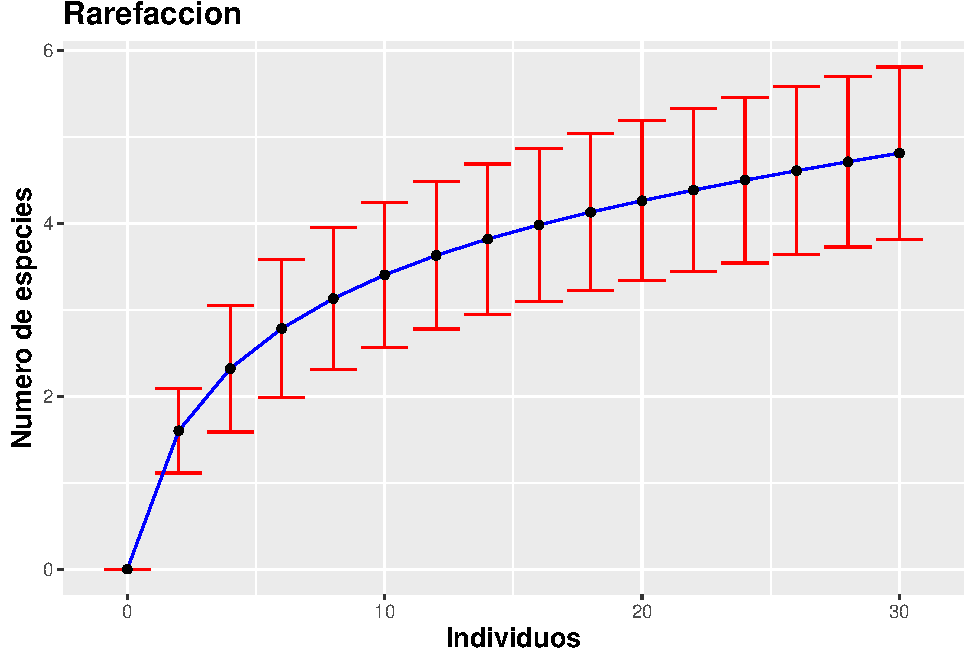
\includegraphics{mangrove_files/figure-latex/unnamed-chunk-5-1.pdf}
\caption{Rarefacción}
\end{figure}

\begin{table}

\caption{\label{tab:unnamed-chunk-6}Índice de valor de importancia}
\centering
\begin{tabular}[t]{l|r|r|r|r}
\hline
Especie & DR & AR & FR & IVI\\
\hline
Prioria copaifera & 0.0740325 & 0.5050505 & 9.090909 & 9.669992\\
\hline
Pelliciera rhizophorae & 0.1592520 & 0.5050505 & 9.090909 & 9.755212\\
\hline
Tabebuia chrysantha & 0.2139538 & 0.5050505 & 9.090909 & 9.809913\\
\hline
Pachira cf. aquatica & 4.5224882 & 3.5353535 & 9.090909 & 17.148751\\
\hline
Raphia taedigera & 7.1183030 & 1.0101010 & 9.090909 & 17.219313\\
\hline
Laguncularia racemosa & 1.9272294 & 1.5151515 & 18.181818 & 21.624199\\
\hline
Montrichardia arborescens & 6.9604198 & 17.6767677 & 9.090909 & 33.728096\\
\hline
Pterocarpus officinalis & 41.5065473 & 16.1616162 & 9.090909 & 66.759073\\
\hline
Rhizophora mangle & 37.5177740 & 58.5858586 & 18.181818 & 114.285451\\
\hline
\end{tabular}
\end{table}

En la \textbf{Tabla IV} se muestra el IVI para todas las especies de las
tres parcelas en estudio, organizado en orden descendente, colocando a
la especie \emph{Rhizophora Mangle} como la más importante de las 3
parcelas aunque no se encuentre en una de ellas(parcela 69), esto puede
atribuirse a la gran dominancia que presenta en las parcelas 62 y 70.
Las otras 2 especies más importantes según el IVI fueron:
\emph{Pterocarpus Officinalis} y \emph{Montrichardia arborescens},
especies que solo se encuentran en la parcela 69, esto puede explicarse
por la gran dominancia que tiene en esta parcela en comparación a las
demás especies de la comunidad, también puede atribuirse a la zonación
que se presenta en la comunidad de las tres parcelas, empezando con una
mayor dominancia de \emph{Rhizophora Mangle} en las parcelas 62 y 70 que
tienen unas condiciones de salinidad de 2.2 ppm y 4.6 ppm
respectivamente y ausencia en la parcela 69. Esto puede deberse a que
esta especie soporta ambientes con alta salinidad e inundación
\citep{AF}, y presenta adaptaciones a estas condiciones, como las raíces
fúlcreas, presencia de neumatóforos (Rhizophora mangle, Instituto
nacional forestal de México) y lenticelas en las raíces para el
intercambio gaseoso de las plantas. Luego avanzando en el paisaje por
medio de las parcelas, se encuentra que \emph{Pterocarpus Officinalis}
tiene una mayor dominancia en la parcela 69 que cuenta con un nivel de
salinidad de 0.8 ppm, esta especie es un árbol de hoja perenne de
contrafuerte grande y relativamente tolerante a la sal \citep{AG}, según
\citep{AH}es particularmente vulnerable al aumento de la salinidad, pues
incrementa las tasas de mortalidad de adultos al tiempo que reduce el
crecimiento, el reclutamiento y la nodulación de la raíz; y finalmente
la especie \emph{Montrichardia arborescens} que es la tercera especie
más importante de la comunidad de las tres parcelas con un IVI de 33.7,
que a pesar de que su dominancia relativa (6.9) es baja respecto a las
otras dos especies mencionadas anteriormente, lo que puede darse a que
\emph{Montrichardia arborescens} habita en ambientes donde la influencia
del mar es baja(poca salinidad) e inundaciones temporales\citep{AI},
aunque según \citep{AI} esta especie presenta adaptaciones morfologicas y
fisiologicas que le permiten crecer en las condiciones de la parcela
69(baja salinidad e inundación moderada). Se puede ver que los
diferentes tipos de salinidad de las parcelas explican la distribución
de las especies y su zonación en la comunidad que iría desde la parcela
70, seguido por la 62 y finalmente con la 69. ya que unas especies están
adaptadas a ambientes más salinos (las de las parcelas 62 y 70) y otras
están adaptadas a lugares con una salinidad baja (las de la parcela 69).

\begin{figure}
\centering
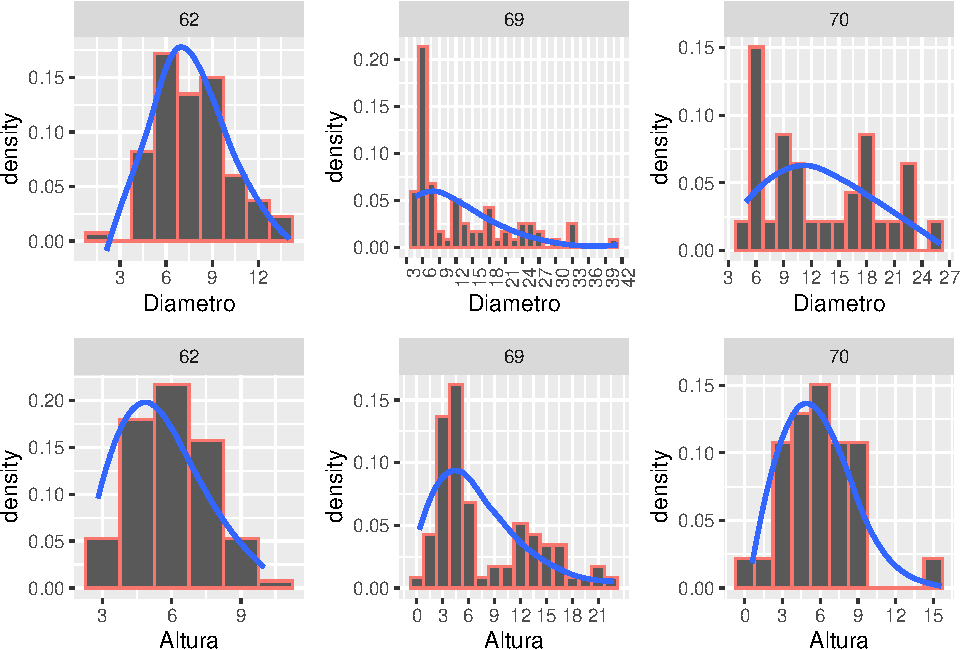
\includegraphics{mangrove_files/figure-latex/unnamed-chunk-13-1.pdf}
\caption{Distribuciónes diamétricas y de alturas}
\end{figure}

En la \textbf{Figura 2} se muestran las distribuciones de diametro (D) y
altura (A), todas estas ajustaron a un modelo tipo ``gamma'' excepto la
parcela 70 que se comportó mejor como ``weibull'' para ambos casos
respectivamente, es evidente notar que hay alturas y diámetros pequeños
para todas las parcelas, sin embargo hay ciertos valores variables que
sugieren diferentes tipos de regeneración, donde la más temprana se
presenta en la parcela 62 pues hay hay una acumulación en los rangos de
6 a 9 cm para D y unos pocos son más grandes algo parecido ocurre con A,
esto quiere decir en este caso que el comportamiento es parecido a un
bosque coetáneo común en plantaciones, esto puede atribuirse a la gran
dominancia de \textbf{Rhizophora Mangle} si bien no es una plantación
las características de dominancia hace que el comportamiento en cuanto a
D y A sea parecido, la misma situación ocurre en la parcela 70 pero acá
el patrón es más evidente en la distribución de A, parece ser que en
este punto de regeneración hay una preferencia de las spp por aumentar
de diametro que en altura (ver anexo 1), lo que podría indicar que no
hay competencia por luz. La tendencia descrita anteriormente no se
cumple con la parcela 69 pues acá hay más variabilidad en los parámetros
de altura y diametro, lo que puede indicar la formación de estratos (ver
anexo 2) es notable la asimetría positiva que presentan las
distribuciones, muy propias de un modelo ``gamma'' \citep{AJ}, la poca
frecuencia que tienen los tamaños grandes indica que hay acceso a la luz
para todas las spp, lo que precisamente hace pensar en estratos del
bosque, muchos árboles pequeños y unos pocos altos o emergentes. Según
esto, es posible intuir que a mayor dominancia de una spp la
probabilidad de encontrar estratos en el bosque será menor.

\href{http://www.scielo.org.co/pdf/prosp/v12n1/v12n1a12.pdf}{anexo}

\bibliography{mybibfile}

\end{document}


